\documentclass[lineno]{biometrika}

\usepackage{amsmath}
%\usepackage{graphics}

%% Please use the following statements for
%% managing the text and math fonts for your papers:
%\usepackage{times}
%\usepackage[cmbold]{mathtime}
%\usepackage{bm}
\usepackage{lipsum}        % lorem ipsum text
\usepackage{booktabs}      % nice tables
\usepackage{tikz}
\usetikzlibrary{shapes.geometric, arrows.meta, positioning}

% define styles
\tikzset{
	process/.style={
		rectangle,
		rounded corners,
		draw=black,
		fill=blue!20,
		text width=3cm,
		align=center,
		minimum height=1cm
	},
	file/.style={
		rectangle,
		draw=black,
		fill=orange!20,
		text width=3cm,
		align=center,
		minimum height=1cm
	},
	arrow/.style={
		->,
		>=Stealth,
		thick
	}
}


\usepackage{newtxtext}
\usepackage[subscriptcorrection]{newtxmath}

%\usepackage{natbib}

\graphicspath{{./art/}}

\usepackage[plain,noend]{algorithm2e}

\makeatletter
\renewcommand{\algocf@captiontext}[2]{#1\algocf@typo. \AlCapFnt{}#2} % text of caption
\renewcommand{\AlTitleFnt}[1]{#1\unskip}% default definition
\def\@algocf@capt@plain{top}
\renewcommand{\algocf@makecaption}[2]{%
  \addtolength{\hsize}{\algomargin}%
  \sbox\@tempboxa{\algocf@captiontext{#1}{#2}}%
  \ifdim\wd\@tempboxa >\hsize%     % if caption is longer than a line
    \hskip .5\algomargin%
    \parbox[t]{\hsize}{\algocf@captiontext{#1}{#2}}% then caption is not centered
  \else%
    \global\@minipagefalse%
    \hbox to\hsize{\box\@tempboxa}% else caption is centered
  \fi%
  \addtolength{\hsize}{-\algomargin}%
}
\makeatother

%%% User-defined macros should be placed here, but keep them to a minimum.
\def\Bka{{\it Biometrika}}

\def\AIC{\textsc{aic}}
\def\T{{ \mathrm{\scriptscriptstyle T} }}
\def\v{{\varepsilon}}

%\addtolength\topmargin{35pt}
\DeclareMathOperator{\Thetabb}{\mathcal{C}}

%\usepackage{hyperref}

\begin{document}

\jname{Biometrika}
%% The year, volume, and number are determined on publication
\jyear{2025}
\jvol{112}
\jnum{1}
\cyear{2025}
%% The \doi{...} and \accessdate commands are used by the production team
%\doi{10.1093/biomet/asm023}
\accessdate{Advance Access publication on 14 February 2025}

%% These dates are usually set by the production team
\received{2 January 2024}
\revised{3 February 2025}

%% The left and right page headers are defined here:
\markboth{DKZ.2R et~al.}{Biometrika style}

%% Here are the title, author names and addresses
\title{Some notes on \textit{Biometrika} style}

\author{Consultants}
\affil{DKZ.2R\\ Aachen
\email{info@dkr2r.de}}


%\author{\and D. M. TITTERINGTON}
%\affil{Department of Statistics, University of Glasgow, Glasgow G12 8QQ, U.K. \email{mike@stats.gla.ac.uk}}

\maketitle

\begin{abstract}
Our paper does not have an abstract. 
\end{abstract}

\begin{keywords}
Address; Appendix; Figure; Length; Reference; Style; Summary; Table.
\end{keywords}

\section{Introduction}

\lipsum[1-2]


\section{Methods}

\lipsum[3]

\subsection{Figures with tikzpicture}


\begin{figure}[http]
	\centering
	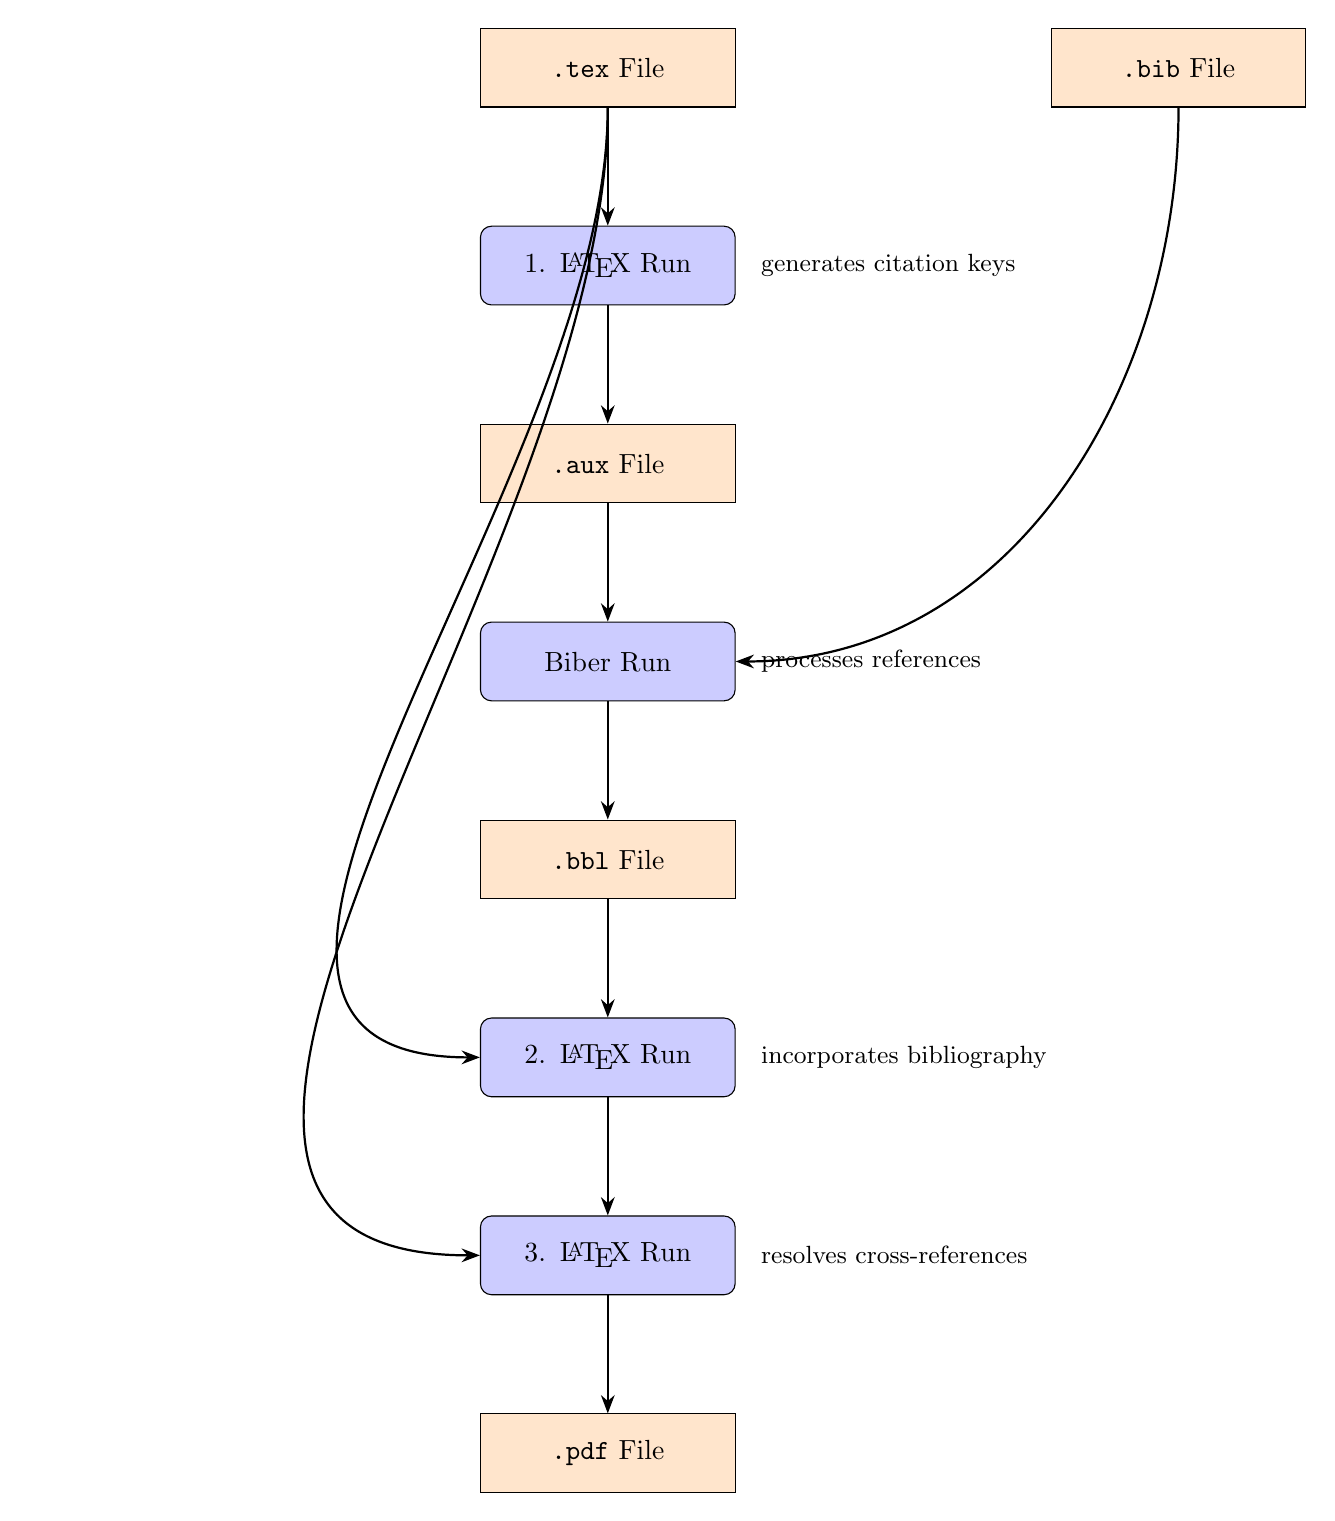
\begin{tikzpicture}[node distance=.25cm]
		
		% nodes
		\node (tex)     [file]                              {\texttt{.tex} File};
		\node (bib)     [file, right=4cm of tex]            {\texttt{.bib} File};
		\node (latex1)  [process, below=1.5cm of tex]       {1. \LaTeX\ Run};
		\node (aux)     [file, below=1.5cm of latex1]       {\texttt{.aux} File};
		\node (biber)   [process, below=1.5cm of aux]       {Biber Run};
		\node (bbl)     [file, below=1.5cm of biber]        {\texttt{.bbl} File};
		\node (latex2)  [process, below=1.5cm of bbl]       {2. \LaTeX\ Run};
		\node (latex3)  [process, below=1.5cm of latex2]    {3. \LaTeX\ Run};
		\node (pdf)     [file, below=1.5cm of latex3]       {\texttt{.pdf} File};
		
		% .tex feeds into all latex runs
		\draw [arrow] (tex) -- (latex1);
		\draw [arrow] (tex.south) to [out=270, in=180] (latex2.west);
		\draw [arrow] (tex.south) to [out=270, in=180] (latex3.west);
		
		% .bib feeds into biber
		\draw [arrow] (bib.south) to [out=270, in=0] (biber.east);
		
		% main flow
		\draw [arrow] (latex1) -- (aux);
		\draw [arrow] (aux)    -- (biber);
		\draw [arrow] (biber)  -- (bbl);
		\draw [arrow] (bbl)    -- (latex2);
		\draw [arrow] (latex2) -- (latex3);
		\draw [arrow] (latex3) -- (pdf);
		
		% annotations
		\node [right=0.2cm of latex1] {\small generates citation keys};
		\node [right=0.2cm of biber]  {\small processes references};
		\node [right=0.2cm of latex2] {\small incorporates bibliography};
		\node [right=0.2cm of latex3] {\small resolves cross-references};
		
	\end{tikzpicture}
	\caption{The LaTeX compilation process with citations using Biber}
	\label{fig:compilation}
\end{figure}


\subsection{Model}

\lipsum[10-11]

\subsection{Data Collection}

\lipsum[4]

\subsection{Unordered List}

The following items were collected:

\begin{itemize}
	\item First item
	\item Second item
	\item Third item
	\begin{itemize}
		\item Nested item 1
		\item Nested item 2
	\end{itemize}
	\item Fourth item
\end{itemize}

\subsection{Ordered List}

The data collection followed these steps:

\begin{enumerate}
	\item First step
	\item Second step
	\item Third step
	\begin{enumerate}
		\item Nested step 1
		\item Nested step 2
	\end{enumerate}
	\item Fourth step
\end{enumerate}


\subsection{Data Analysis}



\lipsum[5]

\section{Results}


\lipsum[6]

\subsection{Table Example}

\begin{table}[h]
	\centering
	\caption{Main table}
	\begin{tabular}{lcc}
		\toprule
		\textbf{Product} & \textbf{Value} & \textbf{Unit} \\
		\midrule
		Product A & 1.00 & kg \\
		Product B & 4.20 & kg \\
		Product C & 3.00 & kg \\
		\bottomrule
	\end{tabular}
	\label{tab:sample}
\end{table}

As shown in Table \ref{tab:sample}, the values increase linearly.


\subsection{Figure Example}

\begin{figure}[h]
	\centering
	% replace with your image
	
\includegraphics[width=0.5\textwidth]{art/my-awesome-image.png}
	\caption{Our main image.}
	\label{fig:sample}
\end{figure}

As shown in Figure \ref{fig:sample}, \lipsum[7]



\section{Conclusion}


\lipsum[10]	

The following conclusions can be drawn:

\begin{enumerate}
	\item Main conclusion
	\item Second conclusion
	\item Maybe we should not use list in the conclusion. 
\end{enumerate}

The importance of clear and effective communication in research cannot be
overstated. As noted by \citep{Graham1995}, even everyday objects such
as the paperclip can serve as a metaphor for the complexity of modern
office life. This insight, combined with the statistical considerations
outlined by \citep{Huff1954}, underlines the need for careful and
transparent reporting of results \citet{Graham1995, Huff1954}.




\newpage

\newpage


\section*{Supplementary material}
\label{SM}
Further material such as technical details, extended proofs, code, for example in \texttt{R} \citep{R:2025}, or additional  simulations, figures and examples may appear online, and should be briefly mentioned as Supplementary Material where appropriate.  Please submit any such content as a PDF file along with your paper, entitled `Supplementary material for Title-of-paper'.
Include in the paper a section `Supplementary material',  with the sentence `The Supplementary Material includes $\ldots$', giving a brief indication of what is available. It should be possible to read and understand the paper without reading the Supplementary Material.



%Further instructions will be given when a paper is accepted.
%\vspace*{-10pt}

\appendix

\appendixone
\section*{Appendix 1}
\subsection*{General}

Any appendices appear after the acknowledgement but before the references, and have titles. If there is more than one appendix, then they are numbered,  as here Theorem~\ref{appthm1}.

\begin{theorem}\label{appthm1}
This is a rather dull theorem:
	\begin{equation}
		\label{A1}
		a + b = b + a;
	\end{equation}
	a little equation like this should only be displayed and labelled if it is referred to elsewhere. 
\end{theorem}


\bibliographystyle{biometrika}
\bibliography{paper-ref}

 


\end{document}\vspace{0.4cm} 
